\documentclass[12pt]{article}
\usepackage{graphicx}

\usepackage{xcolor}
\usepackage{hyperref}
\usepackage{float}
\usepackage{longtable}
%\usepackage{multirow}
%\usepackage{array}
%\newcolumntype{P}[1]{>{\centering\arraybackslash}p{#1}}

\usepackage{xcolor}

\def\xyellowspace{%
  \sbox0{\colorbox{yellow}{\strut\ }}%
  \dimen0=\wd0\relax
  \hskip0pt\cleaders\box0\hskip\dimen0\hskip0pt}

\begingroup
\catcode`\ =\active%
\gdef\makeyellowspace{\let \xyellowspace\catcode`\ =\active}%
\endgroup

\def\?#1{\colorbox{yellow}{\strut#1}}

\newenvironment{evidenzia}
  {\setlength{\fboxsep}{0.2pt}\setlength{\fboxrule}{0pt}%
   \makeyellowspace\ignorespaces}
  {}



\usepackage{blindtext} % to generate dummy text



\usepackage[T1]{fontenc} 							% imposta la codifica dei font
\usepackage[utf8]{inputenc} 							% lettere accentate da tastiera
\usepackage[english]{babel} 							% per scrivere in italiano
\addto{\captionsenglish}{\renewcommand{\bibname}{List of References}}


\usepackage{footmisc}


\usepackage{fancyhdr}
\usepackage{longtable}


\usepackage{subfig}


\usepackage{listings}


\definecolor{mGreen}{rgb}{0,0.6,0}
\definecolor{mGray}{rgb}{0.5,0.5,0.5}
\definecolor{mPurple}{rgb}{0.58,0,0.82}
\definecolor{backgroundColour}{rgb}{0.95,0.95,0.92}

\lstdefinestyle{CStyle}{
    backgroundcolor=\color{backgroundColour},   
    commentstyle=\color{mGreen},
    keywordstyle=\color{magenta},
    numberstyle=\tiny\color{mGray},
    stringstyle=\color{mPurple},
    basicstyle=\footnotesize,
    breakatwhitespace=false,         
    breaklines=true,                 
    captionpos=b,                    
    keepspaces=true,                 
    numbers=left,                    
    numbersep=5pt,                  
    showspaces=false,                
    showstringspaces=false,
    showtabs=false,                  
    tabsize=2,
    language=C
}

\addtolength{\headheight}{1.5cm} % make more space for the header
\pagestyle{fancyplain} % use fancy for all pages except chapter start
\lhead{
\includegraphics[height=0.1cm]{./Images/logo_hidden.png}} % left logo
\rhead{
\includegraphics[height=2.3cm]{./Images/logo.png}} % right logo
\renewcommand{\headrulewidth}{0pt} % remove rule below header

\usepackage[colorinlistoftodos]{todonotes}

\newcommand\tab[1][1cm]{\hspace*{#1}}

\begin{document}

\begin{titlepage}

\newcommand{\HRule}{\rule{\linewidth}{0.5mm}} % Defines a new command for the horizontal lines, change thickness here

\center % Center everything on the page
 
%----------------------------------------------------------------------------------------
%	HEADING SECTIONS
%----------------------------------------------------------------------------------------

\textsc{\LARGE La Sapienza University}\\[1.5cm] % Name of your university/college
\textsc{\Large Department of Computer Science}\\[0.5cm] % Major heading such as course name
\textsc{\large Multimodal Interaction}\\[0.5cm] % Minor heading such as course title

%----------------------------------------------------------------------------------------
%	TITLE SECTION
%----------------------------------------------------------------------------------------

\HRule \\[0.4cm]
{ \huge \bfseries Project Report}\\[0.4cm] % Title of your document
\HRule \\[1.5cm]
 
%----------------------------------------------------------------------------------------
%	AUTHOR SECTION
%----------------------------------------------------------------------------------------

\begin{minipage}{0.4\textwidth}
\begin{flushleft} \large
\emph{Author:}\\
Giordano \textsc{Dionisi} 1834919 

\end{flushleft}
\end{minipage}
~
\begin{minipage}{0.4\textwidth}
\begin{flushright} \large
\emph{Supervisor:} \\
Prof.ssa Maria \textsc{De Marsico} % Supervisor's Name

\end{flushright}
\end{minipage}\\[2cm]

% If you don't want a supervisor, uncomment the two lines below and remove the section above
%\Large \emph{Author:}\\
%John \textsc{Smith}\\[3cm] % Your name

%----------------------------------------------------------------------------------------
%	DATE SECTION
%----------------------------------------------------------------------------------------

{\large \today}\\[2cm] % Date, change the \today to a set date if you want to be precise

%----------------------------------------------------------------------------------------
%	LOGO SECTION
%----------------------------------------------------------------------------------------


\includegraphics[height=3.8cm]{./Images/logo_firstpage.png}\\[3cm] % Include a department/university logo - this will require the graphicx package
 
%----------------------------------------------------------------------------------------

\vfill % Fill the rest of the page with whitespace


\end{titlepage}

\tableofcontents

\newpage

\section{Abstract}

This work proposes the preliminary results of a system to recog-
nize deception from facial microexpressions. Starting from facial
landmarks, the adopted method analyzes the micro-dynamics un-
derlying the facial modifications. This is done both while answering
neutral questions (entailing no reason to lie) and when answering
questions whose responses may cause harm or embarrassment at
least. The preliminary results invite to continue the research of
suitable features to tackle the problem of deception detection.

\section{Introduction}

Several real-world applications beyond pure forensics and court-
room trials, e.g., analysis of video ads, and job interviews, can take
advantage of automatic deception. At present, there are more or
less invasive and demanding methods, especially used in interroga-
tory. The underlying assumption is that physiological measures
can support distinguishing between liars and people telling the
truth. For instance, thermal body imaging can detect the blood
flow via special sensors. Another support comes from voice stress
analysis. Last but not least, the most popular polygraph,
seen in many films, can measures multiple physiological signals at
the same time. These techniques have a twofold disadvantage: a
high cost of the equipment, and the fact that the subjects are almost
always aware of being monitored. This allows, especially to trained
ones, to appropriately modify their behaviour. Also due to the latter
issue, the authors of state that "No machine built to date has
proven more effective than a well-trained human lie detector". On
the contrary, face-based deception detection in video is noninvasive
and moreover the facial images can be captured without the sub-
ject awareness and cooperation, therefore providing more reliable
features to analyze. In fact, psychological studies have assessed
that certain facial micro-actions are difficult to inhibit when the
corresponding facial expression is genuine. In turn, these facial
expressions are equally difficult to counterfeit. In this paper, the
problem of deception detection in face videos is tackled by extract-
ing relevant landmarks from the face, like in, and studying their
dynamics, e.g., eye blinking.

In more specific we have that the system has a very low cost equipment, only a camera, and it has a set of questions. This database is available \_HERE\_ and it's possible see that there are simple questions (for e.g. "what is you name?") but also very and very embarassing questions, like as sessual aspect, personal aspect and so on ("Who is your friend that you prefer?" or "Have you never do a fake orgasm?" and similar things). \\
The person so has to respond to this questions and the system takes into account several features, namely:
\begin{itemize}
    \item Eye Blinking
    \begin{itemize}
        \item Fast Blinking: It sees if the person blinks too high times his eyes. This means that the question isn't too confortable for him and that the probability that he is lying isn't too low, because he's nervous;
        
        \item Slow Blinking: On the other hand also if the person doesn't do a minumum number of blinks, this means that he's lying, in fact this means that the person is doing a forced pose, so he is forced to do the specific expression and he forces all the body and the face to do absolutely nothing to express something with expression. But also no expressions mean a lot;
        
        \item Closed Eyes: For Bouton, if a person closes his eyes for 1-2 seconds, then the probability that he is lying is high, because it is reflecting on what to tell, so he is building a fake answer;
        
        \item Too Opened Eyes: It's possible see if a person is surprised, if its eyes are too opened. In fact this means that our question has upset him.
    
    \end{itemize}
    \item Mouth Movements
    \begin{itemize}
    
        \item Mouth Open: It can mean a surprise, so the person can be embarassed and can tell a fake information, because he did not expect a similar question;
        
        \item Tight Mouth: If person closes a lot his mouth, this means that he's nervous, in fact it's possible perceive his irritation.
        
    \end{itemize}
    
    \item Eyebrows Inarcated: This means "surprise", so the person is embarassed and he didn't expect a similar question. For this reason he is more inclined to not tell the truth;
    
    
    
    \item Position Of Head:
    
    \begin{itemize}
    
        \item Left/Right: For right-hand persons; Someone that looks to right is lying a bit;
        
        \item Bottom Left-Right: For right-hand persons; Someone that looks to right is lying a lot, so it's a big alarm;
        
        \item Tells "No": Unconsciously the person can tell something but he can do a movement with the head like "no". This means that the person himself doesn't believe on what he is telling.
        
    \end{itemize}
    
    \item Distance From Camera: This means that the person wants to take the distances from us, so he wants to go more away possible to avoid to respond to us, in practise.

\end{itemize}

All this is performed by our system to track all micro-expressions on the face. In this way we can obtain an extimate on the probability to tell lies, so it's possible well understand how react to this. 

The important thing than other systems is that the person doesn't know where camera is and he hasn't have someone to talk, so it's more difficult to him to hide his micro-expressions, because he hasn't a reference point and this environment spurs a lot the person to be real with his expressions.

The system generates a plot for each question that the person has to respond, for example:

\begin{figure}[H]

    \includegraphics{./LAYER_AVERAGE__Hai un sogno nel cassetto?.png}

\end{figure}

In this case the question was "do you have a dream in the drawer?"

We have a line for each parameter (for example in violet we have the parameter that measures the amount of "tight mouth") and the most important line is the green line, because it's possible see by means of the legend that this line represents the percentage of lie that the person is telling, frame by frame (more or less 10 frames per second are captured).

Another important line is the "SPEAK" line, because it is the line to tell when the question is finished and, so, when the person can talk.

Combining all this it's possible achieve a good percentage of lies that a person can tell for a specific question and how much things tell his involuntary muscles.

At real time what it's possible see for a real operator is the following:

\begin{figure}[H]

    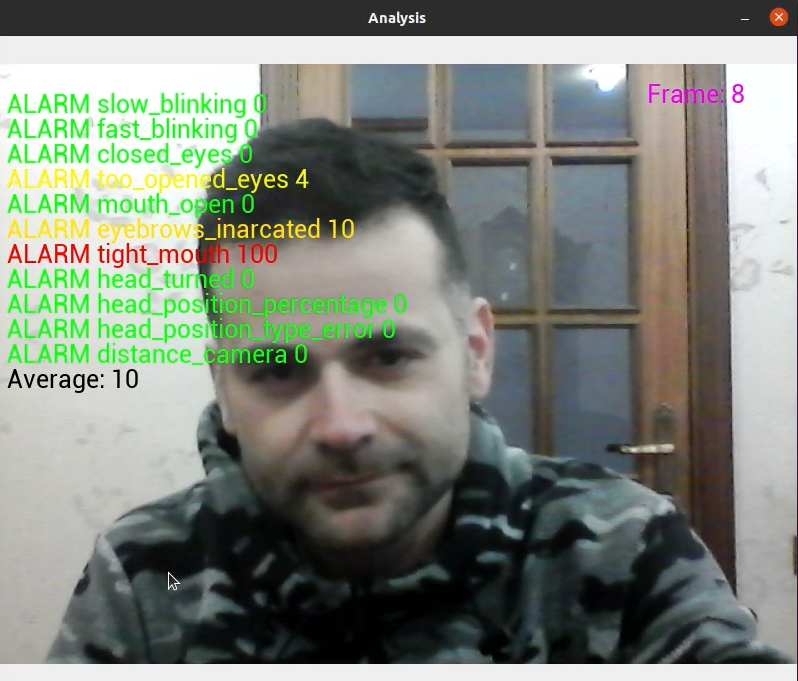
\includegraphics[height=10cm]{./Screenshot.png}

\end{figure}

So it is possible see the average of lie at the bottom in black, the values for each parameter in percentage, the average frame rate in that specific time (higher is better because it's possible catch more micro-aspects) and the face in real-time of the person. So it's enough easy see only the parameters to understand for which parameter the system generates errors, so for which things the person isn't honest and so the probability of lie increases. Higher the percentage of lie and redder become the value, to catch immediately the attention of the operator.

\end{document}
